\documentclass[11pt]{article}

\usepackage{graphicx} 
\usepackage{natbib}

\title{Hausaufgabe 1 \\ Flussproblem}

\author{Jan Niklas Hollenbeck \\ und \\ Marco Leeske}

\date{\today}

\begin{document}

\maketitle

\newpage

\begin{abstract}

Dies wird ein Abstract.Dies wird ein Abstract.Dies wird ein Abstract.Dies wird ein Abstract.Dies wird ein Abstract.Dies wird ein Abstract.Dies wird ein Abstract.Dies wird ein Abstract.Dies wird ein Abstract.Dies wird ein Abstract.Dies wird ein Abstract.Dies wird ein Abstract.Dies wird ein Abstract.Dies wird ein Abstract.Dies wird ein Abstract.Dies wird ein Abstract.Dies wird ein Abstract.Dies wird ein Abstract.Dies wird ein Abstract.Dies wird ein Abstract.Dies wird ein Abstract.Dies wird ein Abstract.Dies wird ein Abstract.Dies wird ein Abstract.Dies wird ein Abstract.Dies wird ein Abstract.Dies wird ein Abstract.Dies wird ein Abstract.Dies wird ein Abstract.Dies wird ein Abstract.Dies wird ein Abstract.Dies wird ein Abstract.Dies wird ein Abstract.Dies wird ein Abstract.Dies wird ein Abstract.Dies wird ein Abstract.Dies wird ein Abstract.Dies wird ein Abstract.Dies wird ein Abstract.Dies wird ein Abstract. 

\end{abstract}


\section{Einleitung}
\label{Einleitung}

Das wird die Einleitung. Das wird die Einleitung. Das wird die Einleitung. Das wird die Einleitung. Das wird die Einleitung. Das wird die Einleitung. Das wird die Einleitung. Das wird die Einleitung. Das wird die Einleitung. Das wird die Einleitung. Das wird die Einleitung. Das wird die Einleitung. Das wird die Einleitung. Das wird die Einleitung. Das wird die Einleitung. Das wird die Einleitung. Das wird die Einleitung. Das wird die Einleitung. Das wird die Einleitung. Das wird die Einleitung. Das wird die Einleitung. Das wird die Einleitung. Das wird die Einleitung. Das wird die Einleitung. Das wird die Einleitung. Das wird die Einleitung. Das wird die Einleitung. Das wird die Einleitung. Das wird die Einleitung. Das wird die Einleitung. Das wird die Einleitung. Das wird die Einleitung. Das wird die Einleitung. Das wird die Einleitung. Das wird die Einleitung. 

%\newpage
%\tableofcontents

\newpage
\section{Einf\"uhrung}
\label{Einfuehrung}

Das Flussproblem beschreibt ein mathematisches Problem in Netzwerken.

\subsection{Algorithmus}
\label{Algorithmus}

Ein Algorithmus beschreibt eine Handlungsvorschrift zur Abarbeitung eines Problems in Einzelschritten. 
\subsection{Algorithmus von Ford und Fulkerson}

\subsection{Algorithmus von Edmonds und Karp}

\subsection{Algorithmus von Dinic}

\subsection{Netzwerke}
\label{Netzwerke}



\subsection{Gerichteter Graph}
\label{Graph}

\begin{figure}[htbp] 
  \centering
     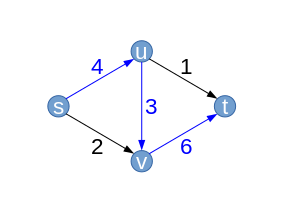
\includegraphics{graph1} 
  \caption{Bild eines Netzwerk-Graphen}
  \label{fig:Graph1}
\end{figure}

\subsection{Netzwerke}
\label{Netzwerke}

\section{Der Inhalt}
\label{Inhalt}

Flussprobleme k\"onnen in Netzwerken mithilfe von Graphen modelliert werden. Hierbei ist ein Quelle-Senke-Netzwerk(im Folgenden q-s-Netzwerk) ein kantenbewerteter, gerichteter Graph G = (V, E) mit der Eigenheit, dass eine Ecke q als Quelle sowie eine Ecke s als Senke bezeichnet wird. Die zwischen Quelle und Senke liegenden Knoten und Kanten können als Zwischenstationen aufgefasst werden. \"Uberdies wird jeder Kante, also eine Verbindung von zwei Ecken im Netzwerk, eine Kapazität c zugewiesen. Sie gibt an, wie viel maximal durch die Kante fließen kann. \citep{Testref}

In Figure \ref{fig:Graph1} unter \ref{Graph} sieht man die Senke auf der linken Seite, gekenn-zeichnet durch "S". 



\section{Experimente}
\label{Experimente}

\subsection{Wirkungsweise der Algorithmen}

\subsection{Laufzeitvergleich}

\subsection{Anwendungszenarien der jeweiligen Algorithmen}

\section{Stand der Technik (Related Work)}
\label{Related Work}
\subsection{Algorithmen und Datenstrukturen Springer Verlag}
\subsection{Graphentheoretische Konzepte und Algorithmen Vieweg und Teubner}

\section{Zusammenfassung}
\label{Zusammenfassung}
\subsection{Ausblick}



\bibliography{test}
\bibliographystyle{plainnat} 

\end{document}
